\documentclass[12pt]{article}

%===============================
%
%          📦 Paquetes
%
%===============================

\usepackage[a4paper, top=2cm, bottom=2cm, left=2.5cm, right=2.5cm]{geometry}
\usepackage[spanish]{babel}
\usepackage[utf8]{inputenc}
\usepackage{amsmath}
\usepackage{multicol}
\usepackage{graphicx}
\usepackage{hyperref}
\usepackage{booktabs}
\usepackage{pgfplots}
\pgfplotsset{compat=1.18}

\title{
  \vspace{2cm}
  \pagenumbering{gobble}
  
\includegraphics[width=5cm]{../assets/logo-utp.png} \\
  \vspace{1cm}
  \textbf{Universidad Tecnológica del Perú} \\
  \vspace{2cm}
  \textbf{Investigación Operativa} \\
  \vspace{1cm}
  \large \textbf{S05 - Evaluación}
}
\author{
  \textbf{Torres Vara, Mateo Nicolas} - \texttt{U24308542} \\
  \texttt{Sección 36373}
}



\begin{document}
\maketitle
\begin{center}

  Docente: Alberto Andre Reyna Alcantara

\end{center}

%======================================
%
%          📚 Inicio del documento
%
%======================================

\newpage
\section*{Ejercicio 1}
\begin{table}[h]
  \centering
  \begin{tabular}{|c|c|c|c|}
  \hline
            & A   & B   & Mínimo \\ \hline
  Calorías  & 180 & 240 & 1600   \\ \hline
  Proteínas & 5   & 8   & 40     \\ \hline
  Precio    & 90  & 120 &        \\ \hline
  \end{tabular}
  \caption{Variables y restricciones}
  \label{tab:Ejercicio1}
\end{table}



\subsection*{Método Gráfico}

\begin{center}
\begin{tikzpicture}
  \begin{axis}[
    axis lines=middle,
    xmin=0, xmax=10,
    ymin=0, ymax=10,
    grid=both,
    xlabel={$x$ (A)},
    ylabel={$y$ (B)},
    width=0.9\linewidth,
    height=0.7\linewidth,
    enlargelimits=false,
    axis equal image,
    legend pos=north east
  ]
  % Calorías: 180x + 240y >= 1600 -> y >= (1600 - 180x)/240
  \addplot[blue, thick, domain=0:8.8] { (1600 - 180*x)/240 };
  \addlegendentry{\( 180x + 240y \geq 1600 \)}

  % Proteínas: 5x + 8y >= 40 -> y >= (40 - 5x)/8
  \addplot[red, thick, domain=0:8] { (40 - 5*x)/8 };
  \addlegendentry{\( 5x + 8y \geq 40 \)}

  % Región factible (gris)
  \fill[gray!30, opacity=0.7]
    (0,6.6667) --
    (0,10) --
    (10,10) --
    (10,0) --
    (8.8889,0) --
    cycle;

  % Puntos factibles (intersección de restricciones)
  \addplot[black, mark=*] coordinates {
    (0,6.6667) 
    (8.8889,0)
  };

  \node at (axis cs:0,6.67) [left] {\((0,6.67)\)};
  \node at (axis cs:0,5) [left] {\((0,5)\)};
  \node at (axis cs:8,0) [below] {\((8,0)\)};
  \node at (axis cs:8.89,0) [below right] {\((8.89,0)\)};
  \end{axis}
\end{tikzpicture}
\end{center}

\[
\begin{array}{l l l l l l l}
180x + 240y \geq 1600 & \rightarrow & 180(0) + 240y = 1600  & \wedge & 180x + 240(0) = 1600 \\
                   &             & y = \dfrac{1600}{240} = 6.67;\; (0,\,6.67) &        & x = \dfrac{1600}{180} = 8.89;\; (8.89,\,0)  \\
                   &             &                    &        &                   \\
5x + 8y \geq 40     & \rightarrow & 0 + y = 5         & \wedge & x + 0 = 8         \\
                   &             & y = 5;\; (0,\,5)   &        & x = 8;\; (8,\,0)  \\
\end{array}
\]

\vspace{0.25cm}

\[
\begin{array}{c c l c l}
\text{Minimizar}\;Z & = & 90x + 120y     &   &      \\
(0;\, 6.67)            & = & 90(0) + 120(6.67) & \approx & 800 \\
(8.89;\, 0)            & = & 90(8.89) + 120(0) & \approx & 800 \\
\end{array}
\]



\newpage
\subsection*{Método Simplex}
\noindent Entre los materiales de clase, no se encuentra información acerca del método simplex para restricciones "mayores o iguales que". Por lo tanto, no he sido capaz de resolver este ejercicio con dicho método a pesar de que he encontrado información de un método bajo el nombre de "Big M" que podría asistir mi problema.



\subsection*{LINGO}
\begin{center}
  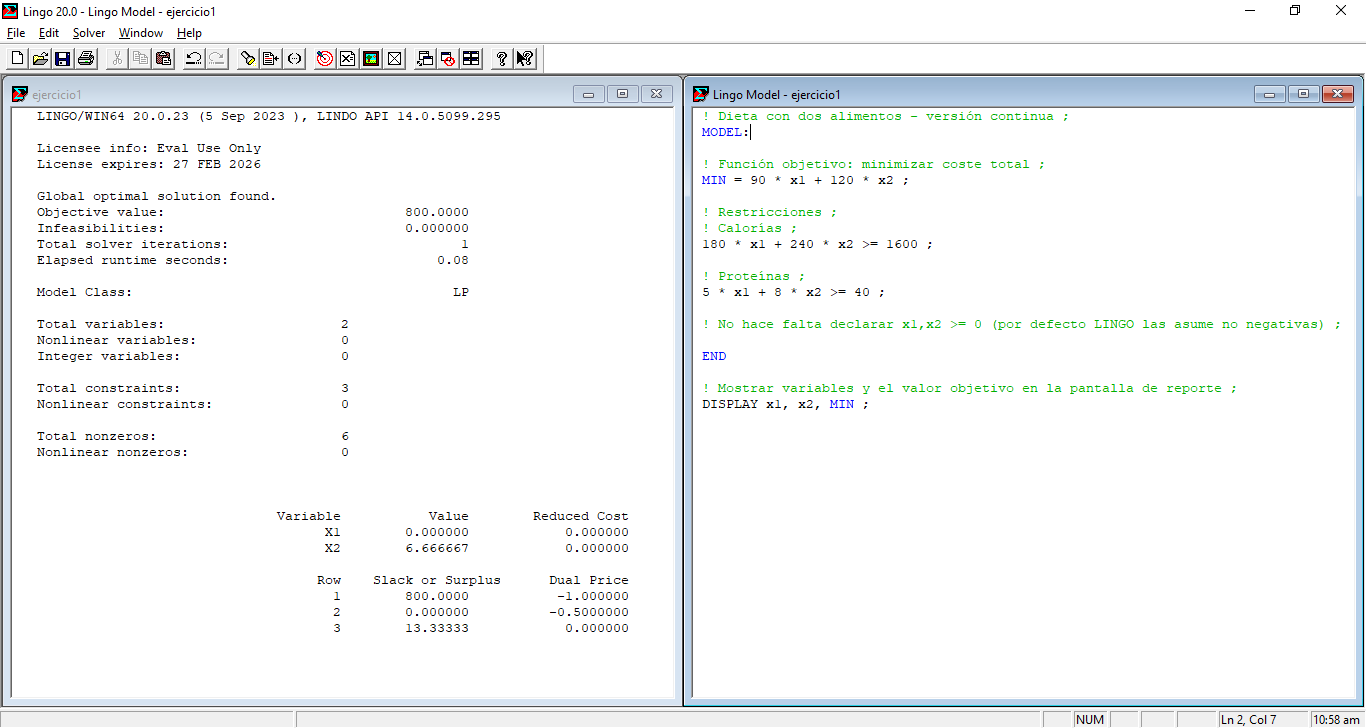
\includegraphics[width=1\textwidth]{./assets/ejercicio1.PNG}
\end{center}

\subsection*{Conclusión}
\noindent El método gráfico da dos posibles resultados óptimos, (0, 6.67) y (8.89, 0), ambos con un costo aproximado de 800 y LINGO toma uno de estos valores como solución óptima (0, 6.67) con un costo de 800. Por lo tanto, el resultado del método gráfico y LINGO coinciden.





\newpage
\section*{Ejercicio 2}

\begin{table}[h]
  \centering
  \begin{tabular}{|c|c|c|c|c|}
  \hline
            & A   & B   & C & Disponibilidad \\ \hline
  Horas Maquinas  & 4.5 & 6.5 & 7 & 480   \\ \hline
  Horas Mano de Obra & 2   & 3  & 5.5 & 90     \\ \hline
  Cantidad    & 1  & 1 & 1 &  \\ \hline
  Beneficio & 120 & 80 & 60 & \\ \hline
  \end{tabular}
  \caption{Variables y restricciones}
  \label{tab:Ejercicio2}
\end{table}

\subsection*{Método Simplex}
\noindent De igual forma que en el ejercicio 1, no he sido capaz de resolver este ejercicio con el método simplex debido a la falta de información acerca de restricciones "mayores o iguales que".
Sin embargo, pude plantear el inicio del problema de la siguiente manera:

\[
\begin{array}{l l l}
4.5x + 6.5y + 7z + S1 & = & 480 \\
2x + 3y + 5.5z + S2 & = & 90 \\
x + y + z - S3 + A1 & = & 100 \\
\text{Maximizar}\;Z & = & 120x + 80y + 60z + 0S1 + 0S2 + 0S3 - MA1\\
\end{array}
\]

\subsection*{LINGO}

\begin{center}
  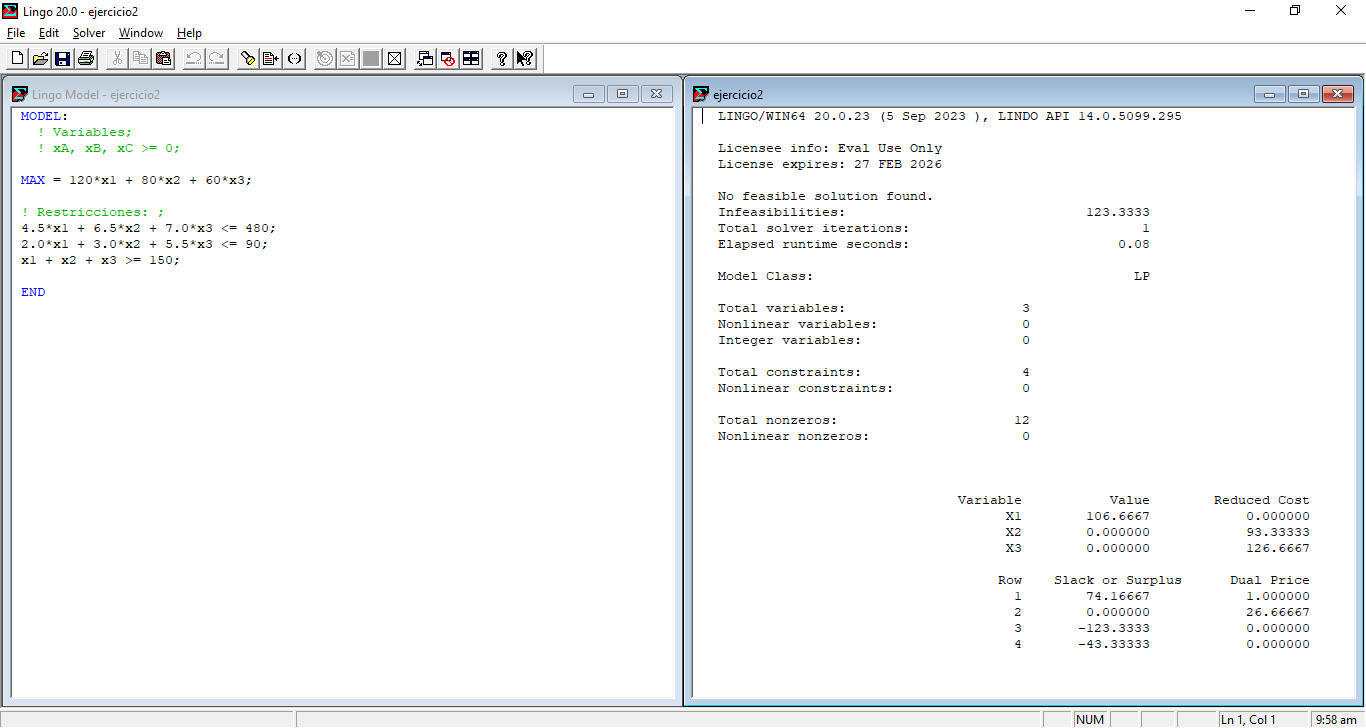
\includegraphics[width=1\textwidth]{./assets/ejercicio2.PNG}
\end{center}

\subsection*{Conclusión}
\noindent Según LINGO no hay una solución factible para este problema.

\newpage
\section*{Recursos y créditos}

\begin{itemize}
    \item \textbf{Código fuente:} \href{https://github.com/MateoTVara/C08-InvestigacionOperativa}{Repositorio GitHub - Investigación Operativa}
    \item \textbf{Carátula por:} \href{https://github.com/1nfinit0}{1nfinit0 en GitHub}
\end{itemize}

\end{document}